\section[Cote 156-8 : les axiomes d'un magasin et le « canular » de la page 102]{Cote 156-8 : les axiomes d'un magasin et le « canular » de la page 102\protect\verifie[\leanblobmain]{Folder156_8}}\label{sec:156-8}

La cote 156-8, chapitre~VIII de \emph{Vers une géométrie des formes}, \q{Analysis situs (quatrième mouture)}, compte cent vingt-six pages datées du 26~juin au 4~juillet 1986. Elle repart des morceaux d'une forme et de trois manières dont deux morceaux se tiennent l'un par rapport à l'autre. Un \emph{magasin} est un ensemble $\mathcal M$ muni d'une \emph{incidence} $X \leq Y$ (\q{$X$ est une strate de $Y$}), d'un \emph{raffinement} $X \ll Y$ (\q{$X$ est contenu dans $Y$}) et d'une \emph{disjonction intérieure} $X \mathrel{|\circ|} Y$ (\q{les intérieurs sont disjoints}). On note $\widetilde X = \{Y \mid Y \leq X\}$. Le modèle à garder en tête est l'ensemble des cellules fermées d'un complexe cellulaire. Les axiomes sont écrits page~7 (\lot{156-8}{1}{7}) :
\begin{itemize}
\item[Mag\,1] $\leq$ et $\ll$ sont des ordres, et $X \leq Y$ entraîne $X \ll Y$ ;
\item[Mag\,2] si $X \ll Y$, les strates $Z \leq Y$ telles que $X \ll Z$ ont un plus petit élément ; on écrit $X \mathrel{\mathring\ll} Y$ (\emph{incidence intérieure}) quand ce plus petit élément est $Y$ ;
\item[Mag\,3] $\mathrel{|\circ|}$ est symétrique et antiréflexive, et $X \mathrel{|\circ|} Y$, $X' \mathrel{\mathring\ll} X$, $Y' \mathrel{\mathring\ll} Y$ entraînent $X' \mathrel{|\circ|} Y'$ ;
\item[Mag\,4] deux strates distinctes d'un même $X$ sont intérieurement disjointes.
\end{itemize}
Deux éléments sont \emph{compatibles}, $X \lessgtr Y$, si toute strate de $X$ qui n'est pas sous $Y$ est intérieurement disjointe de toute strate de $Y$ qui n'est pas sous $X$ : deux cellules qui se touchent au plus le long de faces communes.

Par rapport à la première mouture (cote 156-4, section~\ref{sec:156-4}), le changement est net. Là, la disjonction se déduisait de la compatibilité et de l'absence de minorant commun ; ici la disjonction intérieure est primitive, et c'est la compatibilité qui s'en déduit. Les supports changent avec elle : ils seront définis par la polarité de $\mathrel{|\circ|}$, et non plus par celle de la disjonction.

\subsection*{Premières conséquences (pages 9 et 10)}

Le 27~juin, deux pages intercalaires, numérotées 1bis et 2bis, donnent \q{quelques compléments sur $\mathcal M$ lui-même} (\lot{156-8}{1}{9}, \lot{156-8}{1}{10}). Le bas de la page~9 est un palimpseste de tentatives biffées ; la lecture en dégage la suite suivante.

\begin{encadre}
\begin{theoreme}[Grothendieck, pages 9 et 10, forme de la lecture]
Dans un magasin :
\begin{enumerate}
\item[a)] (prop.~$1_0$) $\lessgtr$ est réflexive et symétrique, et passe aux strates : si $X' \leq X$, $Y' \leq Y$ et $X \lessgtr Y$, alors $X' \lessgtr Y'$ ;
\item[b)] (prop.~2) si $X \neq Y$ et $X \lessgtr Y$, alors $X \mathrel{|\circ|} Y$ ;
\item[c)] (cor.~1 et~2) si $X \lessgtr Y$, $Z \mathrel{\mathring\ll} X$ et $Z \ll Y$, alors $X \leq Y$ ; si de plus $Z \mathrel{\mathring\ll} Y$, alors $X = Y$ ;
\item[d)] (cor.~3) si $X \lessgtr Y$, alors $X \ll Y$ équivaut à $X \leq Y$ ;
\item[e)] (prop.~3) $\mathring\ll$ est réflexive et transitive ;
\item[f)] (NB de la page~10) si $X \ll Y \ll Z$ et $X \mathrel{\mathring\ll} Z$, alors $Y \mathrel{\mathring\ll} Z$.
\end{enumerate}
\end{theoreme}
\end{encadre}

\begin{proof}
Deux remarques que la page laisse implicites servent partout. D'abord $\mathring\ll$ est réflexive : si $Z \leq X$ et $X \ll Z$, Mag\,1 donne $Z \ll X \ll Z$, donc $Z = X$. Ensuite, si $X \ll Y$, le plus petit élément $Y'$ de Mag\,2 vérifie $Y' \leq Y$ et $X \mathrel{\mathring\ll} Y'$.

a) La réflexivité est vide, la symétrie vient de celle de $\mathrel{|\circ|}$. Soient $X'' \leq X'$ hors de $\widetilde{Y'}$ et $Y'' \leq Y'$ hors de $\widetilde{X'}$ ; ils sont distincts. Si $X''$ est sous $Y$, ce sont deux strates distinctes de $Y$, et Mag\,4 conclut ; de même si $Y''$ est sous $X$ ; sinon, c'est la définition de $X \lessgtr Y$.

b) Si aucun des deux n'est sous l'autre, c'est la définition de la compatibilité, appliquée à $X$ et $Y$ eux-mêmes ; si $X < Y$, ce sont deux strates distinctes de $Y$, et Mag\,4 conclut.

c) Soit $Y' \leq Y$ avec $Z \mathrel{\mathring\ll} Y'$. Par a), $X \lessgtr Y'$. Si $X \neq Y'$, b) donne $X \mathrel{|\circ|} Y'$, et Mag\,3, avec $Z \mathrel{\mathring\ll} X$ et $Z \mathrel{\mathring\ll} Y'$, donne $Z \mathrel{|\circ|} Z$, contre l'antiréflexivité. Donc $X = Y' \leq Y$. Si de plus $Z \mathrel{\mathring\ll} Y$, on a de même $Y \leq X$.

d) On applique c) avec $Z = X$.

e) Si $X \mathrel{\mathring\ll} Y \mathrel{\mathring\ll} Z$, alors $X \ll Z$, et il existe $Z' \leq Z$ avec $X \mathrel{\mathring\ll} Z'$. Si $Z' \neq Z$, Mag\,4 donne $Z' \mathrel{|\circ|} Z$, Mag\,3 donne $X \mathrel{|\circ|} Y$, puis $X \mathrel{|\circ|} X$ : absurde. Donc $Z' = Z$.

f) Si $W \leq Z$ et $Y \ll W$, alors $X \ll W$, donc $W = Z$.
\end{proof}

En Lean, les axiomes sont la structure \texttt{IsMagasin}, et les énoncés a) à f) sont \texttt{compat\_mono}, \texttt{dis\_of\_compat}, \texttt{le\_of\_compat\_of\_intLe}, \texttt{eq\_of\_compat\_of\_intLe}, \texttt{ref\_iff\_le\_of\_compat}, \texttt{intLe\_trans} et \texttt{intLe\_of\_ref\_of\_ref}.

La page écrit deux de ces énoncés sous une forme plus forte, et la formalisation confirme les deux corrections de la lecture. Le modèle est celui de deux segments du plan, $X = [p,q]$ et $Y = [r,s]$, dont l'extrémité $q$ tombe à l'intérieur de $Y$. Le magasin a six éléments : quatre points et deux segments, avec $q \ll Y$ et $q \mathrel{\mathring\ll} Y$ ; tous les couples distincts sont intérieurement disjoints, sauf $q$ et $Y$.

\begin{encadre}
\begin{contrexemple}[Énoncés de la page, marge de la page~9 et corollaire~3 transcrit]
Ce modèle vérifie Mag\,1 à Mag\,4. On y a $X \neq Y$ et $X \mathrel{|\circ|} Y$, mais $X$ et $Y$ ne sont pas compatibles : la réciproque \q{si $X \neq Y$, $X \mathrel{|\circ|} Y \Leftrightarrow X \lessgtr Y$} de la marge de la page~9 est fausse. On y a aussi $p \lessgtr X$ et $p \leq X$, sans $p \mathrel{\mathring\ll} X$ : le corollaire~3 tel que la transcription le porte, \q{$X \lessgtr Y$ entraîne $X \mathrel{\mathring\ll} Y \Leftrightarrow X \leq Y$}, est faux ; il est vrai avec $\ll$.
\end{contrexemple}
\end{encadre}

\begin{proof}
L'intérieur ouvert de $X$ ne rencontre pas celui de $Y$, mais le point $q$, strate de $X$ qui n'est pas sous $Y$, n'est pas intérieurement disjoint de $Y$, strate de $Y$ qui n'est pas sous $X$. Pour le second énoncé, $p$ n'a pas de strate hors de $\widetilde X$, donc $p \lessgtr X$ ; et le plus petit $Z \leq X$ avec $p \ll Z$ est $p$, non $X$. Les axiomes et les deux calculs sont vérifiés par énumération dans le noyau (\texttt{twoSegments\_isMagasin}, \texttt{twoSegments\_not\_compat}, \texttt{twoSegments\_cor3\_as\_transcribed}).
\end{proof}

Le NB de la page~10 ajoute que, dans f), on n'a pas nécessairement $X \mathrel{\mathring\ll} Y$, et Grothendieck le montre par un dessin : un segment $Y$ dans un segment $Z$, et l'extrémité $X$ de $Y$, intérieure à $Z$ (figure~\ref{fig:156-8-nb}). Le dessin est lui aussi un magasin à six éléments ; la formalisation vérifie les axiomes, puis $X \ll Y \ll Z$, $X \mathrel{\mathring\ll} Z$, $Y \mathrel{\mathring\ll} Z$ et non $X \mathrel{\mathring\ll} Y$ (\texttt{subSegment\_isMagasin}, \texttt{subSegment\_nb}).

\begin{figure}[ht]
\centering
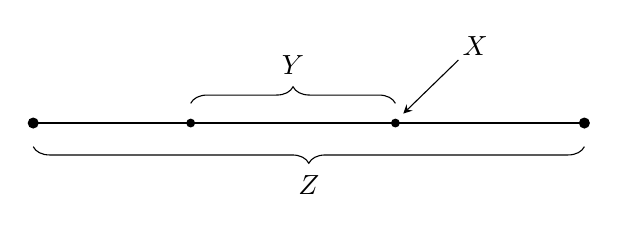
\begin{tikzpicture}[x=1cm,y=1cm]
\draw[line width=1pt] (0,0) -- (7,0);
\foreach \x in {0,7} \fill (\x,0) circle (2pt);
\foreach \x in {2,4.6} \fill (\x,0) circle (1.6pt);
\draw[decorate, decoration={brace, amplitude=6pt}] (2,0.25) -- (4.6,0.25) node[midway, above=7pt] {$Y$};
\draw[decorate, decoration={brace, amplitude=6pt, mirror}] (0,-0.3) -- (7,-0.3) node[midway, below=7pt] {$Z$};
\draw[->, >=stealth] (5.4,0.8) node[above right=-2pt] {$X$} -- (4.7,0.12);
\end{tikzpicture}
\caption{Le NB de la page~10 : $X \ll Y \ll Z$ et $X \mathrel{\mathring\ll} Z$, donc $Y \mathrel{\mathring\ll} Z$, mais $X$ est une strate de $Y$ et l'on n'a pas $X \mathrel{\mathring\ll} Y$. Figure de l'édition, redessinée d'après le croquis de la page, un segment gradué sous deux accolades et une flèche (\lot{156-8}{1}{10}).}
\label{fig:156-8-nb}
\end{figure}

\subsection*{Le magasin d'un ensemble ordonné et ses supports (pages 89 à 102)}

Le premier juillet, Grothendieck associe un magasin à tout ensemble ordonné $L$ (\lot{156-8}{5}{89}). Ses éléments sont les \emph{points} $P_x$, $x \in L$, et les \emph{intervalles} $S_{a,b}$, $a < b$ ; les strates de $S_{a,b}$ sont $P_a$, $P_b$ et lui-même, et la disjonction intérieure est
\[
P_x \mathrel{|\circ|} P_y \iff x < y \text{ ou } y < x, \qquad
P_x \mathrel{|\circ|} S_{a,b} \iff x \leq a \text{ ou } b \leq x, \qquad
S_{a,b} \mathrel{|\circ|} S_{a',b'} \iff b \leq a' \text{ ou } b' \leq a .
\]
Pour une partie $\Phi$ de $\mathcal M$, le \emph{cosupport intérieur} $\mathrm{cosupp}^\circ(\Phi)$ est l'ensemble des éléments intérieurement disjoints de tous ceux de $\Phi$, et le \emph{support intérieur} est $\mathrm{supp}^\circ(\Phi) = \mathrm{cosupp}^\circ(\mathrm{cosupp}^\circ(\Phi))$. C'est la polarité de la relation symétrique $\mathrel{|\circ|}$, la même construction qu'à la cote 156-4 pour une autre relation. Comme $\mathrel{|\circ|}$ est antiréflexive, $\Phi \subset \mathrm{supp}^\circ(\Phi)$ et $\mathrm{supp}^\circ(\Phi) \cap \mathrm{cosupp}^\circ(\Phi) = \emptyset$ : aucun élément n'est disjoint de lui-même.

Pour calculer les supports, la page~99 pose une hypothèse (\lot{156-8}{5}{99}) :
\q{si $L$ n'a pas de plus petit élément, alors pour tout $a \in L$, existe $x \in L$ tel que $x < a$}, et l'énoncé dual. C'est l'hypothèse~H. Le lemme~1 affirme alors que le support d'un élément est son ombre, $\mathrm{supp}^\circ(\widetilde X) = \mathrm{Omb}(X) = \{Z \mid |Z| \subset |X|\}$, avec $|P_x| = \{x\}$ et $|S_{a,b}| = [a,b]$. Le corollaire~1 en est le cas d'un point (\lot{156-8}{5}{100}).

\begin{encadre}
\begin{theoreme}[Grothendieck, pages 99 à 101, lemme~1 pour un point]
Soit $L$ un ensemble ordonné qui vérifie l'hypothèse~H. Pour tout $a \in L$, $\mathrm{supp}^\circ(\{P_a\}) = \{P_a\}$.
\end{theoreme}
\end{encadre}

\begin{proof}
Soit $X$ dans le support. Il n'est pas intérieurement disjoint de $P_a$, sans quoi il serait aussi dans le cosupport. Si $a$ est un plus petit élément, tout autre point $P_z$ vérifie $a < z$ et tout intervalle $S_{c,d}$ vérifie $a \leq c$ : tous sont disjoints de $P_a$, donc $X = P_a$. Le cas d'un plus grand élément est symétrique. Sinon, l'hypothèse~H donne $x < a < y$ : comme $a$ n'est pas un plus petit élément, ou bien $L$ en a un, qui est un minorant strict de $a$, ou bien la seconde branche de H en fournit un ; de même pour $y$. Les intervalles $S_{x,a}$ et $S_{a,y}$ sont disjoints de $P_a$, donc $X$ est disjoint des deux. Si $X = P_z$, on a $z \leq x$ ou $a \leq z$, puis $z \leq a$ ou $y \leq z$ ; $z \leq x$ et $y \leq z$ rendraient $P_z$ disjoint de $P_a$, donc $z = a$. Si $X = S_{c,d}$, la disjonction d'avec $S_{x,a}$ donne $a \leq c$ ou $d \leq x < a$, et dans les deux cas $S_{c,d}$ serait disjoint de $P_a$ (\lot{156-8}{6}{101}). En Lean, c'est \texttt{supp\_pt}, pour tout ensemble ordonné.
\end{proof}

Page~102, Grothendieck essaie de voir ce qui se passe sans~H, sur l'ensemble à trois éléments $a < b > c$ ($a$ et $c$ incomparables), dont le magasin a cinq éléments $P_a, P_b, P_c, S_{a,b}, S_{c,b}$ (\lot{156-8}{6}{102}). Il trouve
\[
\mathrm{cosupp}^\circ(P_b) = \mathcal M \smallsetminus \{P_b\}, \quad
\mathrm{cosupp}^\circ(\{P_a\}) = \{P_b, S_{a,b}, S_{c,b}\}, \quad
\mathrm{supp}^\circ(\{P_a\}) = \{P_a, P_b\} \neq \{P_a\},
\]
puis $\mathrm{cosupp}^\circ(\widetilde S_{a,b}) = \emptyset$ et $\mathrm{supp}^\circ(\widetilde S_{a,b}) = \mathcal M \neq \mathrm{Omb}(S_{a,b})$, et il écrit dans la marge \q{Canular}, lu avec doute.

\begin{center}
\begin{tikzpicture}[x=1.2cm,y=1cm]
\node (a) at (0,0) {$a$};
\node (c) at (2,0) {$c$};
\node (b) at (1,1) {$b$};
\draw (a) -- (b) -- (c);
\end{tikzpicture}
\end{center}

\begin{encadre}
\begin{contrexemple}[Calcul de la page~102]
Pour l'ensemble ordonné $a < b > c$, $\mathrm{cosupp}^\circ(\{P_a\}) = \{P_b, S_{a,b}\}$ et $\mathrm{supp}^\circ(\{P_a\}) = \{P_a\}$ : la conclusion du corollaire~1 reste vraie, bien que $L$ ne vérifie pas l'hypothèse~H. Ce qui est juste dans la page, c'est le cas d'un intervalle : $\mathrm{cosupp}^\circ(P_b) = \mathcal M \smallsetminus \{P_b\}$, $\mathrm{cosupp}^\circ(\widetilde S_{a,b}) = \emptyset$ et $\mathrm{supp}^\circ(\widetilde S_{a,b}) = \mathcal M$, alors que $\mathrm{Omb}(S_{a,b}) = \widetilde S_{a,b} = \{P_a, P_b, S_{a,b}\}$. Le lemme~1 tombe donc en défaut pour les intervalles.
\end{contrexemple}
\end{encadre}

\begin{proof}
$P_a$ n'est pas intérieurement disjoint de $S_{c,b}$, puisque $a$ n'est ni $\leq c$ ni $\geq b$ ; ni de $P_c$, qui lui est incomparable. Le cosupport de $\{P_a\}$ est donc $\{P_b, S_{a,b}\}$. Le point $P_b$, qui n'est pas disjoint de lui-même, ne peut être dans le support. $P_c$ n'est pas disjoint de $S_{a,b}$, ni $S_{c,b}$ de $S_{a,b}$ : il reste $P_a$. Pour $\widetilde S_{a,b}$, un élément disjoint de $P_a$, $P_b$ et $S_{a,b}$ devrait être hors de $\{P_a, P_b, S_{a,b}\}$, mais $P_c$ n'est pas disjoint de $P_a$, ni $S_{c,b}$ de $S_{a,b}$ : le cosupport est vide, et le cosupport du vide est $\mathcal M$. Enfin $[a,b] = \{a, b\}$ ne contient pas $c$, d'où l'ombre. En Lean, les supports sont calculés sur des parties finies (\texttt{cosuppF}, \texttt{suppF}, qui coïncident avec les définitions générales par \texttt{coe\_suppF}), et les égalités sont vérifiées par énumération : \texttt{can\_cosupp\_pa}, \texttt{can\_supp\_pa}, \texttt{can\_cosupp\_pb}, \texttt{can\_supp\_segment}, \texttt{can\_not\_hypH}.
\end{proof}

\begin{remarque}
L'hypothèse~H ne peut pas pour autant être retirée du corollaire~1 : pour deux éléments incomparables $a$ et $c$, le magasin n'a que deux points, qui ne sont pas disjoints, et $\mathrm{supp}^\circ(\{P_a\}) = \{P_a, P_c\}$ (\texttt{anti\_supp\_pa}). La page~102 avait donc le bon diagnostic, que H sert, mais sur le mauvais élément : l'exemple $a < b > c$ défait le lemme~1 pour $S_{a,b}$, non pour $P_a$.
\end{remarque}

Ne sont pas démontrés ici : que le magasin d'un ensemble ordonné vérifie Mag\,1 à Mag\,4 (page~91), les modèles finis les vérifiant seuls ; le lemme~1 et ses corollaires~2 à~4 pour un intervalle sous l'hypothèse~H ; les propriétés des pages~92 et~93 (divisibilité, fidélité ssi $L$ totalement ordonné) ; la description des figures finies par les drapeaux de drapeaux (pages~97 et~98).
